
\begin{section}{Experimentación}
 No se realizaron estudios in vitro, comparando la simulación contra un fluido real bajo las mismas condiciones. Se realizaron dos videos uno es un \href{https://www.youtube.com/watch?v=D8JOELu8uAs}{mapa de velocidad total codificado por color}, donde el color codifica la velocidad y el otro un \href{https://www.youtube.com/watch?v=_JisfmOIEdU}{campo vectorial}
 campo vectorial donde cada flecha representa la velocidad y dirección del fluido en cada punto. La simulación parece reflejar el comportamiento esperado por un fluido. No se realizaron mas estudios cualitativos.
~\\
~\\
Fueron realizados estudios de rendimiento, tratando de medir el impacto de la ejecución en paralelo. Como marco teórico de esta sección, se utilizó por un lado la Ley de Amdahl, midiendo así el speedup  $S(n,p) = \frac{T_{ser}(n) }{ T_{par}(n,p)}$  a trabajo fijo aumentando la cantidad de procesadores, y por otro la Ley de Gustavson para la cual medimos el trabajo realizado por cantidades cada vez mas grandes de recursos de procesamiento a tiempo constante, y luego calculamos la eficiencia $E(n,p) = \frac{S(n,p)}{p}$. Donde $ T_{ser}(n)$  es el tiempo que tarda el programa en su versión serial para una entrada de tamaño n, y $T_{par}(n,p)$  es el tiempo que tarda el programa paralelo para una entrada de tamaño n y cantidad de procesos p.

\begin{subsection}{Ley de Amdahl}
~\\
La Ley de Amdahl nos da el speedup teórico en la ejecución de una tarea que consta de una cantidad de trabajo fijo al incrementar los recursos del sistema.
~\\
~\\
Llevada al limite, sirve para calcular la mejora máxima posible para una tarea que consta de una parte paralelizable, y una parte serial que no puede ser efectivamente paralelizada.
~\\
La formulación matemática de la Ley de Amdahl es la siguiente:
~\\
~\\
\begin{center}
$S(s) \leq  \frac{1}{(1-p)+\frac{p}{s}}$
\end{center}
~\\
~\\
Donde S es el speedup total, s el speedup de la parte del programa que se favorece por el paralelismo, y p es la proporción de tiempo que era ocupada por la parte del programa que tiene speedup alguno. Se asume que todo el tiempo que no corresponde a p, o sea 1-p, se mantiene igual. Un resultado directo de esta ley es que incluso utilizando infinitos recursos, no puede aumentarse el speedup mas que:

~\\
~\\
\begin{center}
$S(s) \leq  \frac{1}{1-p}$
\end{center}
~\\
~\\
\newpage
Para este experimento se quiere dejar fija la cantidad de trabajo total realizado, y medir como cambia la velocidad al agregar unidades de procesamiento. 
~\\
~\\
El programa fue ejecutado en una red ethernet con 21 maquinas, cada una disponiendo de 4 núcleos. Al momento de realizar la experimentación, estas maquinas estaban siendo utilizadas, a razón de dos nucleos por maquina, con lo cual se disponía de 42 núcleos para procesar la prueba. Los resultados son los siguientes:
~\\
\begin{verbatim}
nucleos time
30      43.681s
25      45.017s
20      49.776s
15      56.197s
12      69.997s
10      82.439s
9       94.491s
8       102.819s
6       142.737s
5       171.753s
3       343.118s
1       867.247s
\end{verbatim}
~\\
Con lo cual los speedups serían:
~\\
\begin{verbatim}
nucleos speedup

30      0.050367427
25      0.051907934
20      0.0573954133
15      0.0647993017
12      0.0807117234
10      0.0950582706
9       0.1089551189
8       0.1185579195
6       0.1645863289
5       0.1980439252
3       0.3956404577
1       1
\end{verbatim}

En el siguiente gráfico se pueden ver los datos de la tabla.
~\\
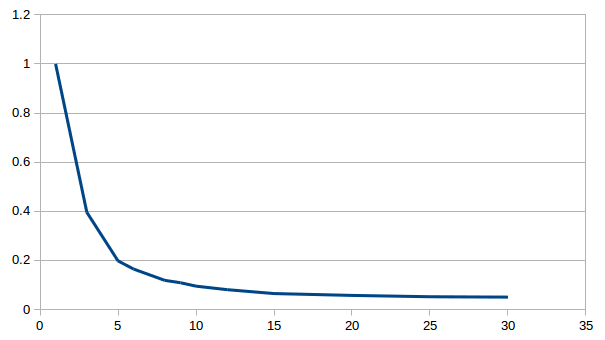
\includegraphics{AmdahlSpeedup}

Como puede apreciarse, el speedup tiende hacia una asintota horizontal, en la cual se encuentra la sección serial del programa. El mejor speedup que se pudo conseguir fue de 0.050367427.
\end{subsection}


\begin{subsection}{Ley de Gustavson}
~\\
La Ley de Gustafson calcula el speedup teórico para una tarea de tiempo de ejecución fijo al incrementar los recursos de un sistema. Al aplicar la Ley de Gustavson, lo que varia no es el tiempo de ejecución, sino la cantidad de trabajo realizado. 
~\\
La formulación matemática de la Ley de Gustavson es la siguiente:
~\\
~\\
\begin{center}
$S(s) = p - \alpha(p-1)$
\end{center}
~\\
~\\
Donde S es el speedup, p es el número de procesadores, y $\alpha$ la parte no paralelizable del proceso. Notar que si se aumenta notablemente la el trabajo total en la sección paralelizable, haciendo que la proporción de trabajo serial $\alpha$ sea muy pequeña, esto resulta en algo muy similar a $S(s) = p$


En este experimento se quiere dejar el tiempo limite en 120s, y medir cuanto trabajo pudo realizarse para distintas cantidades de unidades de procesamiento.
~\\
~\\ 
El programa fue nuevamente ejecutado en una red ethernet con 21 maquinas, cada una disponiendo de 4 núcleos. Al momento de realizar la experimentación, estas maquinas estaban siendo utilizadas, a razón de un núcleo por maquina, con lo cual se disponía de 63 núcleos para procesar la prueba. 
~\\
~\\
Medir la cantidad de trabajo que se utilizó para la versión paralela, en la versión serial resultó prohibitivo, por lo cual no se dispone de una medida de tiempo serial para la misma cantidad de trabajo que la utilizada en las mediciones sobre el programa paralelo. Por esto ultimo no fue posible hacer una medición de eficiencia. Aún así se pretende obtener una medida sobre el rendimiento del paralelizado realizado. Para eso se contó la cantidad de elementos del sistema calculados, que al fin y al cabo es lo que nos interesa calcular. Es importante aclarar que cuando en la tabla de resultados figura que se utilizó un solo núcleo, esa medición fue realizada sobre la versión serial del programa, no perdiendo así tiempo en inicializar las variables de MPI, calcular las secciones, y otras cuestiones que no son necesarias ne la versión serial. Por comodidad, la unidad de medida elegida para medir el trabajo fue millones de elementos calculados. Los resultados son los siguientes:
~\\
\begin{verbatim}
núcleos   trabajo
1         111.113
5         413.814
20        1976.24
35        3198.04
50        3661.31
60        4294.03
\end{verbatim}

Estos se comportan linealmente, como puede verse en el siguiente gráfico:

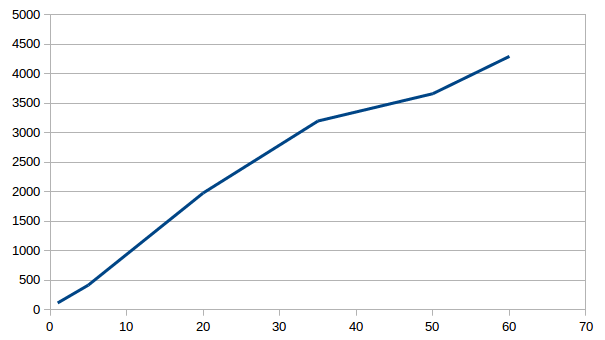
\includegraphics{Gustavson}

Si calculamos el trabajo realizado por cada núcleo obtenemos:
\begin{verbatim}
núcleos   trabajo/núcleos
1         111.113
5         82.7628
20        98.812
35        91.3725714286
50        73.2262
60        71.5671666667
\end{verbatim}

Y finalmente dividiendo este valor por el trabajo realizado por un núcleo, obtenemos una medida de cuanto trabajo logramos extraer por núcleo, al compararlo con una versión serial.
\newpage
\begin{verbatim}
núcleos   trabajo/(núcleos*111.113)
1         1
5         0.7448525375
20        0.889292882
35        0.8223391631
50        0.6590245966
60        0.6440935504
\end{verbatim}
El siguiente es el gráfico correspondiente a estos valores:

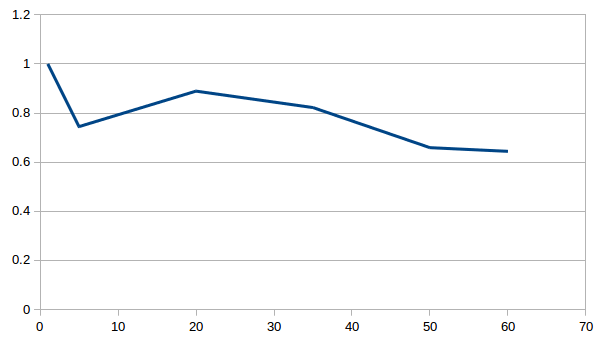
\includegraphics{Gustavson2}

 Vemos en si bien la gráfica se veía lineal, la pendiente era menor a uno, y el trabajo realizado es claramente menor que el resultado de multiplicar la cantidad de núcleos por el trabajo que es capaz de realizar la versión serial.
 A pesar de esto, se puede ver que se puede aumentar la cantidad de trabajo realizable de forma lineal agregando unidades de procesamiento, lo cual es un resultado mas optimista que el planteado por la Ley de Amdahl.

\end{subsection}
\end{section}

